\documentclass[titlepage, 12pt]{scrartcl}

\usepackage[utf8]{inputenc}

\usepackage{amsmath,amssymb,amsthm}
\usepackage{thmtools}

\usepackage[croatian]{babel}
\usepackage{csquotes}

\usepackage[unicode]{hyperref}
\usepackage{enumitem}
\usepackage{minted}
\usepackage{graphicx}

\usepackage[style=numeric]{biblatex}
\addbibresource{literatura.bib}

\MakeOuterQuote{"}


\title{Modeliranje grafovske baze podataka za društvenu mrežu - \emph{Neo4j}}
\author{Karlo Basioli \and 
	Antonela Bogdanić \and 
	Ivan Krcivoj }
\date{Lipanj 2021}

\makeatletter         
\def\@maketitle{
	\raggedright
	\includegraphics[width = 40mm]{logo.jpg}\\[8ex]
	\begin{center}
		{\Huge \bfseries \sffamily \@title }\\[4ex] 
		{\Large  \@author}\\[4ex] 
		
		\includegraphics[width = 40mm]{image.png}
		
		\@date\\[8ex]
\end{center}}

\makeatother

\begin{document}
	
	\begin{titlepage}
		
		\newcommand{\HRule}{\rule{\linewidth}{0.5mm}}
		\center
		\textsc{\Large Prirodoslovno-matematički fakultet}\\[1.5cm] % Name of your university/college
		\textsc{\large Matematički odsjek}\\[0.5cm] % Major heading such as course name
		\textsc{\large Napredne baze podataka}\\[0.5cm] 
		
		\HRule \\[0.4cm]
		{ \Large \bfseries Modeliranje grafovske baze podataka za društvenu mrežu - \emph{Neo4j}}\\[0.4cm] 
		\HRule \\[1.5cm]
		
		
		\begin{minipage}{0.4\textwidth}
			\begin{flushleft} \large
				\emph{Autori:}\\
				Karlo \textsc{Basioli} \\
				Antonela \textsc{Bogdanić} \\
				Ivan \textsc{Krcivoj}
			\end{flushleft}
		\end{minipage}
		~
		\begin{minipage}{0.4\textwidth}
			\begin{flushright} \large
				\emph{Mentor:} \\
				Ognjen \textsc{Orel} % Supervisor's Name
			\end{flushright}
		\end{minipage}\\[2cm]
		
		{\large Lipanj 2021}\\[2cm] 
		
		
\includegraphics[scale=0.8]{slike/pmf_logo.jpg}\\
		
		\vfill 
		
	\end{titlepage}
	
	\tableofcontents
	
	\newpage
	
	\section{Uvod}
	
	Tema ovog projekta je modeliranje grafovske baze podataka za društvenu mrežu koristeći \emph{Neo4j}. Zadatak podrazumijeva odabir programskog jezika za izgradnju grafičkog sučelja, osmišljavanje i implementaciju struktura podataka potrebnih za pisanje kompleksnih upita te generiranje podataka i punjenje same baze. \\
	Projekt smo u potpunosti izveli koristeći \emph{Python 3.9} programski jezik uz modul \emph{tkinter} za grafičko sučelje i modul \emph{neo4j} koji omogućava spajanje na bazu. \\
	U sklopu projekta trebali smo osmisliti upit za predlaganje osoba sličnih po obrazovanju i znanju te upit za predlaganje osoba po samostalno osmišljenom kriteriju.
	
	\newpage
	\section{Struktura podataka}
	Prvi problem projekta je razrada struktura podataka kojima će društvena mreža biti modelirana. Kao inspiracija poslužile su nam društvene mreže kao što su \emph{Facebook}, \emph{Twitter}, \emph{Instagram}, \emph{LinkedIn} \dots \\
	Ove popularne društvene mreže danas broje stotine milijuna korisnika. Unatoč brojnim razlikama u suštini imaju sličnu poantu. Njihova zadaća je povezati korisnike. Ljudi koji koriste ove mreže mogu se međusobno dodavati za prijatelje, pratiti razne grupe, razmjenjivati poruke, dijeliti fotografije i slično. \\
	Aspekt koji je gotovo uvijek zajednički je upravo spajanje korisnika. To će biti fokus ovog projekta. Trebamo osmisliti kako reprezentirati korisnika i njegove veze sa ostalim korisnicima. Također moramo ih smisleno podijeliti po edukaciji i njihovim vještinama. \\
	Grafovska baza sastavljena je od vrhova koji predstavljaju osobe i fakultete u danoj bazi te relacije koje predstavljaju njihove odnose.
	
	\subsection{Vrhovi}
	\subsubsection{Person}\label{sec:Person}
	Korisnik će u bazi podataka biti reprezentiran vrhom \emph{Person} sa sljedećim svojstvima:
	\begin{itemize}
		\begin{samepage}
			\item \textbf{id} identifikacija korisnika
			\item \textbf{name} ime korisnika
			\item \textbf{surname} prezime korisnika
			\item \textbf{gender} spol korisnika
			\item \textbf{date\_of\_birth} datum rođenja korisnika
			\item \textbf{skills} vještine koje korisnik dobija samostalno ili učenjem na fakultetu
			\item \textbf{hobbies} hobiji korisnika
		\end{samepage}
	\end{itemize}
	Svaki \emph{id} postavljen je prilikom generiranja koda te je postavljen kao jedistven u bazi naredbom:
	%TODO vidi kako ovo popraviti
	\begin{samepage}
		\begin{minted}[tabsize=1,breaklines]{java}
			CREATE CONSTRAINT personIdConstraint ON (person:Person) ASSERT person.id IS UNIQUE;
		\end{minted}
	\end{samepage}
	Zbog jednostavnosti prijave korisnika u aplikaciju kombinacija (\emph{name}, \emph{surname}) je jedinstvena za svakog korisnika.
	\\ \\
	\subsubsection{College}
	Kako je važno znati edukaciju korisnika, u bazi podataka nalaziti će se i vrh \emph{College} koji predstavlja fakultet te ima sljedeća svojstva:
	\begin{itemize}
		\begin{samepage}
			\item \textbf{id} identifikacija korisnika
			\item \textbf{name} puno ime fakulteta
			\item \textbf{short\_name} skraćeno ime fakulteta
			\item \textbf{area} područje u koje spada fakultet
			\item \textbf{skills} vještine koje polaznik ovog fakulteta može steći
		\end{samepage}
	\end{itemize}
	Slično kao kod vrha \emph{Person} svojstvo \textbf{id} je jedinstveno. \\
	Važna pretpostavka ove baze je da je svaki njen korisnik pohađao fakultet. 
	\subsection{Relacije}
	\subsubsection{IS\_FRIEND}
	Očito važna relacija u ovoj bazi podataka je relacija \emph{IS\_FRIEND}. Ova relacija uspostavlja se između dva vrha sa oznakom \emph{Person} i ukazuje na to da su ta dva korisnika prijatelji u ovoj društvenoj mreži. \\
	Jedini atribut je:
	\begin{itemize}
		\begin{samepage}
			\item \textbf{start\_date} početak prijateljstva
		\end{samepage}
	\end{itemize}
	Veza nije usmjerena te između dva korisnika postoji najviše jedna ovakva veza. \\ \\
	
	\begin{figure}[h]
		\centering
		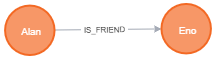
\includegraphics[scale=0.7]{slike/IS_FRIEND.png}
		\caption{Relacija \emph{IS\_FRIEND}}
		\label{fig:friendship}
	\end{figure}
	
	\subsubsection{SAME\_AREA}
	Relacija \emph{SAME\_AREA} povezuje dva fakulteta koja spadaju u isto znanstveno područje. Ona služi za lakše povezivanje osoba sličnog obrazovanja. \\
	Veza također nije usmjerena te dva fakulteta mogu biti povezana najviše jednom ovakvom vezom. \\
	U konkretnoj bazi postoje samo tri područja.
	\\ \\
	\begin{figure}[h]
		\centering
		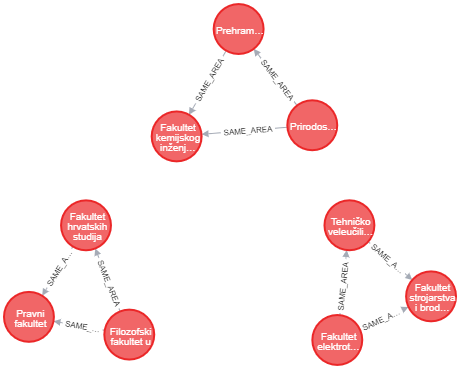
\includegraphics[scale=0.7]{slike/SAME_AREA.png}
		\caption{Relacija \emph{SAME\_AREA}}
		\label{fig:area}
	\end{figure}
	
	\subsubsection{ATTENDED}
	Na kraju postoji i relacija \emph{ATTENDED}. Ovo je prva i jedina usmjerena relacija u bazi. Predstavlja vezu između korisnika i fakulteta. Ukoliko se ova dva vrha povezana bridom \emph{ATTENDED} to znači da korisnik pohađa ovaj fakultet. \\
	Svojstva ove veze su:
	\begin{itemize}
		\begin{samepage}
			\item \textbf{enrollment\_year} godina upisa fakulteta
			\item \textbf{graduate\_year} godina završetka fakulteta
			\item \textbf{grade} prosjek ocjena dosadašnjeg studija
		\end{samepage}
	\end{itemize}
	\begin{figure}[h]
		\centering
		
\includegraphics[scale=0.7]{slike/ATTENDED.png}
		\caption{Relacija \emph{ATTENDED}}
		\label{fig:attendance}
	\end{figure}
	\newpage
	
	\section{Generiranje podataka}
	Nakon što smo osmislili strukturu podataka koju ćemo koristiti bilo je potrebno stvoriti podatke kako bismo napunili našu bazu podataka. Htjeli smo da generirani podaci budu realni kako bi što bolje reprezentirali stvarni svijet. Prilikom odabira skupa podataka na temelju kojih smo generirali bazu obratili smo pozornost da ne budu previše raznoliki ali opet dovoljno bogati da bi lakše i kvalitetnije testirali upite na bazu.
	\subsection{Izvori podataka}
	Na internetskoj stranici \cite{imena} nalazi se popis s gotovo tisuću petsto imena kojima je pridružena oznaka spola kojem ime pripada. Popis prezimena preuzeli smo s internetske stranice \cite{prezimena}.
	Kod odabira fakulteta koje će pohađati izmišljeni korisnici odlučili smo se razmatrati fakultete koji su dio Sveučilišta u Zagrebu. Kako bi podaci bili zanimljiviji odabrali smo po tri fakulteta iz tri različita područja znanosti. Područja kojima fakulteti pripadaju su:
	\begin{itemize}
		\item Prirodoslovni
		\item Društveni
		\item Tehnički
	\end{itemize}
	Fakultete koje smo odabrali za svako područje možete vidjeti na slici \ref{fig:area}.
	Za svaki fakultet napisali smo niz vještina koje osoba može steći njegovim pohađanjem.
	Za kraj smo osmislili neki skup hobija kojima bi se korisnici mogli baviti.
	\subsection{Kako su podaci generirani}
	Kada smo prikupili i osmislili podatke bilo ih je potrebno pridružiti \emph{vrhovima} i \emph{bridovima}.
	
	Imena i prezimena su na jedinstven način pridruživana osobama kako bi očuvali integritet baze.
	
	Datum rođenja odabrali smo na slučajan način između 1980.\ i 2000.\ godine. Za taj raspon smo se odlučili kako bi svi korisnici bili punoljetni te mogli pohađati fakultet.
	
	Za odabir broja hobija i vještina koje korisnik posjeduje koristili smo normalnu distribuciju.
	\newpage
	\begin{figure}[h]
		\centering
		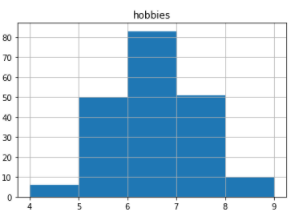
\includegraphics{slike/Hobbies_distribution.png}
		\caption{Distribucija hobija}
		\label{fig:hobbies}
	\end{figure}
	
	\begin{figure}[h]
		\centering
		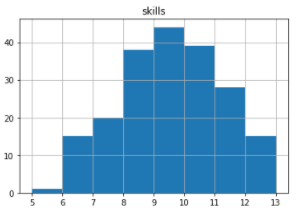
\includegraphics{slike/Skills_distribution.png}
		\caption{Distribucija vještina}
		\label{fig:skills}
	\end{figure}
	Kod odabira vještina pobrinuli smo se da većina vještina bude povezana s fakultetom kojeg osoba pohađa ili je pohađala a, manji broj bude ne vezan uz fakultet. Na primjer student PMF-a može biti vješt u pisanju filmskih kritika iako je to vještina koja se obično stječe na društvenim fakultetima.
	
	Svaka osoba u prosjeku ima 10 nasumično odabranih prijatelja. Datum početka prijateljstva je nasumično odabran od trenutka kad su obje osobe napunile 18 godina do danas.
	
	Svaka osoba pohađa ili je pohađala slučajno odabrani fakultet. Osoba je fakultet upisala nakon što je napunila 18 godina i završila ga je u roku od 5 do 10 godina. Ukoliko osoba još nije završila fakultet u \emph{graduate\_year} navodi godinu kada planira završiti fakultet.
	
	Ocjena je decimalni broj između dva i pet zaokružen na dvije decimale. Vrijednost ocjene koju osoba ima dolazi iz normalne distribucije ali, ovisi i o broju vještina koje posjeduje. Ukoliko osoba posjeduje više vještina veće su šanse da ima bolju ocjenu.
	\begin{figure}[h]
		\centering
		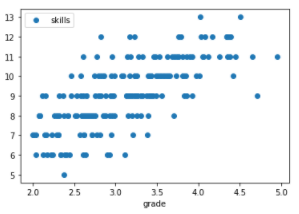
\includegraphics{slike/Grades.png}
		\caption{Ovisnost ocjene o broju vještina}
		\label{fig:hobbies}
	\end{figure}
	
	Funkcije koje stvaraju upravo opisane podatke nalaze se u datoteci \emph{db\_create.py}. 
	Te funkcije stvorene podatke zapisuju u \emph{.csv} datoteke kako bi ih kasnije mogli učitati u bazu podataka.  
	\newpage
	
	\section{Implementacija aplikacije i grafičko sučelje}
	Kao što je već spomenuto za izgradnju aplikacije koristili smo programski jezik \emph{Python} zbog velikog broja modula koje posjeduje i jednostavnosti korištenja tih modula. \\
	Za interakciju sa bazom korišten je modul \emph{neo4j} dok se grafičko sučelje izgradilo s modulom \emph{tkinter}.
	\subsection{Modul neo4j}
	Među nekoliko postojećih \emph{Python} modula za \emph{Neo4j} odabrali smo modul \emph{neo4j}. Ovaj modul podržan je od strane \emph{Neo4j} baze podataka što stoji i u dokumentaciji \cite{neo4j-python}.\\
	Za projekt je napravljena klasa \emph{Database} kao \emph{singleton} kako se ne bi nepotrebno stvarao preveliki broj različitih \emph{drivera}.
	
	\begin{samepage}
		\begin{minted}[tabsize=1,breaklines]{python}
			class Database:
			__instance = None
			
			@staticmethod
			def get_instance(path = "database.cfg"):
			if Database.__instance == None:
			Database(path)
			return Database.__instance
			
			def __init__(self, path):
			if Database.__instance != None:
			raise Neo4jError("This class is a singleton!")
			else:
			#čitanje potrebnih podataka iz .cfg datoteke
			self.driver = GraphDatabase.driver(db_url, auth=(username, password))
			Database.__instance = self
			
			def close(self):
			self.driver.close()
		\end{minted}
	\end{samepage}
	Prikazane su samo najosnovnije metode ove klase. \\
	Instanca ove klase koristi se za slanje upita na bazu podataka. Jednostavan uzorak koji je praćen kroz cijeli projekt izgleda otprilike ovako:
	\begin{samepage}
		\begin{minted}[tabsize=1, breaklines]{python}
			def query_database(cypher_query, args_dict, path_to_cfg):
			db = Database.get_instance(path_to_cfg)
			
			with db.driver.session() as session:
			result = session.run(cypher_query, args_dict)
			#obrada dobijenih rezultata
		\end{minted}
	\end{samepage}
	\
	Veliki izazov korištenja ovog modula i projekta općenito bilo je osmisliti kako puniti bazu sa generiranim podacima. Kao što je već spomenuto generirani podaci spremani su u \emph{.csv} datoteke. \\
	Deklarativni jezik \emph{cypher} podržava naredbu: 
	\begin{minted}{java}
		LOAD CSV
	\end{minted}
	Ova naredba omogućava jednostavno učitavanje \emph{.csv} datoteka. Kako bi bilo omogućeno što jednostavnije punjenje baze za različite korisnike ove datoteke se pokretanjem \emph{Python} skripte šalju u \emph{import} direktorij čiji je \emph{path} potrebno zapisati u \emph{database.cfg} datoteku. \\
	Upiti za učitavanje vrhova iz baze grade se na sljedeći način:
	\begin{samepage}
		\begin{minted}[tabsize=1,breaklines]{python}
			def get_load_command_entity(self, file_name, header, entity):
			header = header.split(",")
			cypher = f"LOAD CSV WITH HEADERS FROM \"file:///{file_name}\" AS csv_line CREATE (p:{entity}" + "{"
				first = True
				
				for header_element in header:
				if first:
				cypher += add_attribute(header_element)
				first = False
				else:
				cypher += ", " + add_attribute(header_element)
				
				cypher += "});"
			
			return cypher
		\end{minted}
	\end{samepage}
	Na ovaj način osigurano je jednostavno punjenje baze podataka za svakog korisnika pokretanjem skripti za generiranje podataka, a potom i skripte za punjenje baze.
	\subsection{Tkinter}
	
	Aplikacija kojom ćemo demonstirati rad društvene mreže i korištenje opisane baze podataka napisana je u \emph{Pythonu} uz korištenje modula \emph{tkinter}. \emph{Tkinter} je jedan od najčešće korištenih i najjednostavnijih modula za izradu grafičkog sučelja za aplikacije pisane u \emph{Pythonu}. Kako u fokusu našeg zadatka nije grafičko sučelje, nećemo previše ulaziti u detalje, no proći ćemo kroz najvažnije dijelove koda i opisati najkorištenije elemente.  
	
	Kratki slijed korištenja ovog modula glasi ovako: uvezi modul \emph{tkinter}, stvori prozor na kojem se kasnije smještaju ostali elementi uz pomoć \mintinline{python}{Tk()}, dodaj elemente po želji i akcije vezane na te elemente. 
	
	
	Važniji elementi koje koristimo u ovoj aplikaciji su:
	\begin{itemize}
		\item \mintinline{python}{Button} - gumb, klikom na gumb pozivaju se druge funkcije/događaji
		\item \mintinline{python}{Radiobutton} - specijalizirani gumb, služi za odabir točno jedne ponuđene vrijednosti
		\item \mintinline{python}{Listbox} - specijalizirani gumb, služi za odabir više ponuđenih vrijednosti
		\item \mintinline{python}{Label} - \emph{display box} u koji stavljamo tekst
		\item \mintinline{python}{Frame} - \emph{display box} u koji dodajemo druge elemente za lakše uređenje prozora ili obavljanje istih operacija na elementima unutar njega - njegovoj djeci
		\item \mintinline{python}{Scrollbar} - element koji služi da unutar prozora imamo manji prozor s mogućnosti \emph{skrolanja} po vrijednostima zapisanim unutra
		\item \mintinline{python}{Entry} - služi za upisivanje vrijednosti korisnika
		\item \mintinline{python}{Calendar}\footnote[1]{Potrebno je pokrenuti naredbu \mintinline{python}{pip install tkcalendar}} - služi za korisnikov unos datuma rođenja, moguće je kretati se po mjesecima i godinama i označiti dan
	\end{itemize}
	
	
	Lijep primjer na kojem vidimo opisane elemente možete proučiti na slici~\ref{fig:forma}.
	
	\begin{figure}[h]
		\begin{center}
			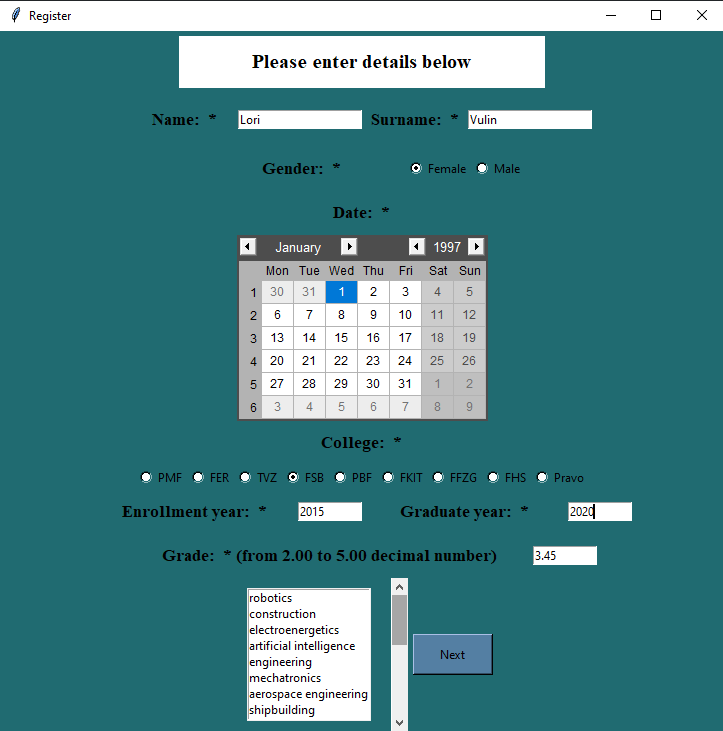
\includegraphics[scale = 0.7]{slike/forma.png}
			\caption{Register window s formom za unos podataka}
			\label{fig:forma} 
		\end{center}
	\end{figure}
	
	
	Parametri koje pozivamo prilikom stvaranja elemenata određuju svojstva elementa poput roditelja, boje pozadine, boje slova, fonta, veličine, naslova... Ta svojstva možemo mijenjati i pozivanjem metode \mintinline{python}{.configure(svojstvo=vrijednost)}.
	
	Također, koristimo i \emph{tkinterov} \mintinline{python}{StringVar} u kojem spremamo vrijednosti koje vraćaju elementi koji očekuju korisnikov unos. 
	
	Postoji više načina za postavljanje elemente na određene pozicije na prozoru ili unutar drugih elemenata. Mi smo se odlučili koristiti metodu \mintinline{python}{pack()} na elementu koja smješta \emph{widgete} u blokove prije smještanja istih u roditeljski \emph{widget}. Taj način nam je bio pogodan obzirom na izgled ostalih prozora koje imamo u aplikaciji. Sa \mintinline{python}{side=lokacija} postavljamo element na neku od pozicija koje su LEFT, RIGHT, TOP, BOTTOM, a s \mintinline{python}{padx} ili \mintinline{python}{pady} podešavamo \emph{padding}. 
	
	Svojstvo gumba da bude onemogućen u nekim situacijama pokazalo nam se jako koristno pri izradi aplikacije. U dijelu aplikacije želimo blokirati mogućnosti korisnika da ponovo klikne na gumb i pozove funkciju. Način na koji to blokiramo je pozivanje: \mintinline{python}{button.configure(state = DISABLED)}.
	
	Cijela funkcinalnost aplikacije zasniva se na korištenju opisanih elemenata uz dodatnu metodu koja omogućuje interaktivnost, a to je metoda \mintinline{python}{destroy()}.\ Ona uništava prozor ili element na kojem ju pozivamo, kao i svu njegovu djecu. Spomenut ćemo i korisnost \mintinline{python}{lambda} funkcija koje nam pomažu pri slanju argumenata među funkcijama koje se pozivaju klikom na gumb. 
	
	Stvaranje prozora i nekih elemenata na njemu opisat ćemo na dijelu koda koji se poziva prilikom pokretanja aplikacije. 
	
	\begin{samepage}
		\begin{minted}[tabsize=1,breaklines]{python}
			def main_window():
			global main_screen
			main_screen = Tk()
			main_screen.geometry("500x250")
			main_screen.title("Account Login")
			main_screen.configure(bg='#acc4d7')
			Label(text="Select Your Choice", 
			bg="white", width=30, height=2, 
			font=("Times", 15, "bold")
			).pack(side=TOP, pady=40)
			
			Button(text="Log in", bg="#547fa3", 
			height=2, width=20, command=login
			).pack(side=LEFT, padx=50)
			
			Button(text="Register",bg="#547fa3", 
			height=2, width=20, command=register
			).pack(side=RIGHT, padx=50)
			
			main_screen.mainloop()
		\end{minted}
	\end{samepage}
	
	Aplikacija se pokreće pozivom prikazane funkcije. Tada se otvara prozor koji je stvoren koristeći \mintinline{python}{Tk()}. Zadnja metoda koju pozivamo na definiranom prozoru je \mintinline{python}{mainloop()} koja se poziva kada je prozor "spreman" za korištenje i kao što joj i ime kaže, beskonačno se vrti sve dok je prozor otvoren, čeka na događaje ili gašenje. Izgled prozora iz primjera vidite na slici~\ref{fig:main}. 
	
	\begin{figure}[h]
		\begin{center}
			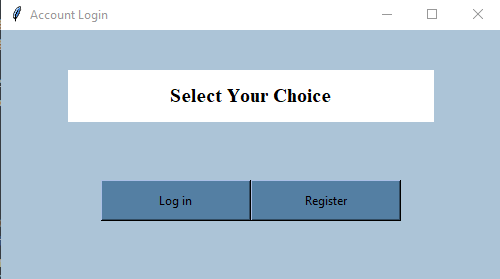
\includegraphics[scale=0.8]{slike/main.png}
			\caption{Početni prozor aplikacije}
			\label{fig:main} 
		\end{center}
	\end{figure}
	
	
	\newpage
	
	\section{Preporuke}
	Postoje različiti načina stvaranja preporuka korisniku. Mnoge društvene mreže korisne razne alate i strojno učenje kako bi smislili najbolje moguće preporuke svojim korisnicima.
	Neke od ovih društvenih mreža nerijetko se nalaze i u problemima s privatnosti zbog iznenađujuće preciznih preporuka.
	Postoje mišljenja da ti algoritmi koriste informacije za koje korisnik nikad eksplicitno ne da dopuštenje kao što je lokacija. \\
	Ovaj projekt srećom koristi generirane podatke te izbjegava probleme privatnosti. Cilj nije složiti model koji će učiti preferencije korisnika već iskoristiti grafovsku strukturu podataka kako bi po vezama između korisnika mogli dati što bolju preporuku po predodređenim kriterijima. \\
	Slijede neke, možda očite, metode preporučivanja zaključno sa implementacijom naših algoritama preporučavanja.
	
	\subsection*{Preporuke po broju zajedničkih prijatelja}
	Najjednostavniji način za dobiti preporuku je poprilično izravan. Korisnik za preporuku dobija upravo one ljude s kojima ima najviše zajedničkih prijatelja. \\
	U bazi \emph{neo4j} sljedećim upitom moguće je dobiti zajedničke prijatelje dva korisnika:
	\begin{samepage}
		\begin{minted}[tabsize=1,breaklines]{java}
			MATCH (p:Person {id:72})-[i:IS_FRIEND]-(common:Person)-[j:IS_FRIEND]-
			(potential_friend:Person {id: 83}) 
			WHERE p.id <> potential_friend.id AND NOT ((p)-[:IS_FRIEND]-(potential_friend)) 
			RETURN p, common, potential_friend,i,j;
		\end{minted}
	\end{samepage}
	\begin{figure}[h]
		\centering
		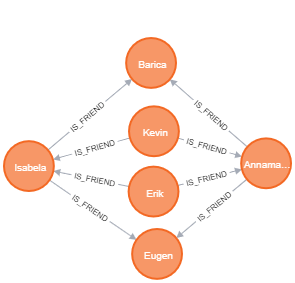
\includegraphics[scale=0.7]{slike/common_friends_query.png}
		\caption{Zajednički prijatelji}
		\label{fig:common_friends}
	\end{figure}
	
	\subsection*{Preporuke po utjecaju}
	Slično kao u prethodnom primjeru i ovdje dolazi do preporuke po zajedničkim prijateljima. Ipak, u ovoj metodi situacija je nešto drugačija. \\
	Pretpostavimo da imamo korisnika \emph{p} i korisnika \emph{potential\_friend} koji imaju zajedničke prijatelje, ali nisu međusobno prijatelji. \\
	Pretpostavimo da su njihovi zajednički prijatelji $commons = \{c_1, c_2, \dots, c_n\}$ za koje je $friends\_num(c_i)$ jednak broju prijatelja koje korisnik $c_i$ ima. \\
	Što korisnik $c_i$ ima manji broj prijatelja smatran je korisnikom koji je selektivniji u izboru svojih prijatelja. Ponekad ima smisla da veću težinu donosi selektivnija osoba zato što je izglednije da ima osobnu vezu sa korisnikom. \\
	Korisniku $potential\_friend$ dodjeljuje se ocjena izračunata kao suma recipročnih vrijednosti $friends\_num(c_i)$ gdje su $c_i$ zajednički prijatelji korisnika $p$ i korisnika $potential\_friend$. \\
	Formula za izračun ocjene izgleda ovako:
	\begin{equation*}
		rating(potential\_friend) = \sum_{c \in commons} \frac{1}{friends\_num(c)}
	\end{equation*}
	Osoba sa najvećim \emph{ratingom} bit će prva preporuka po ovom algoritmu. \\
	Dobro je primjetiti da je razlomak u gornjem izrazu uvijek dobro definiran pošto svaki korisnik $c$ ima barem dva prijatelja s obzirom na to da da je on zajednički prijatelj korisnicima $p$ i $potential\_friend$. \\
	Slijedi upit kojim bi se izračunao \emph{rating} korisnika u \emph{cypheru}.
	
	\begin{samepage}
		\begin{minted}[tabsize=1,breaklines]{java}
			MATCH (p:Person {id:72})-[:IS_FRIEND]-(common:Person)-[:IS_FRIEND]-
			(potential_friend:Person {id: 83}) 
			WHERE p.id <> potential_friend.id AND NOT ((p)-[:IS_FRIEND]-(potential_friend)) 
			WITH common, potential_friend
			MATCH (common)-[r:IS_FRIEND]-(:Person)
			WITH COUNT(r) AS friends_num, common, potential_friend
			RETURN SUM(1.0/friends_num) AS rating, potential_friend;
		\end{minted}
	\end{samepage}
	
	\subsection*{Klasifikacijske preporuke}
	Ovakav tip preporuka gleda zajednička svojstva dva korisnika i na temelju toga donosi odluku tko je kome najsličniji. \\
	Za ovu bazu zajedničko svojstvo korisnika može biti fakultet koji oba korisnika pohađaju, a moguće ih je poredati po broju istih vještina koje imaju. Ovakva preporuka ima smisla zato što je logično da će se ljudi sa istog fakulteta poznavati te da je veća vjerojatnost da će se željeti sprijateljiti ako su njihove vještine slične. \\
	\newpage
	Primjer upita koji prikazuje sve studente na jednom fakultetu:
	
	\begin{samepage}
		\begin{minted}[tabsize=1,breaklines]{java}
			MATCH (p:Person)-[att:ATTENDED]->(c:College {short_name: "TVZ"})
			RETURN p, c, att LIMIT 10;
		\end{minted}
	\end{samepage}
	
	Rezultat istog upita:
	\begin{figure}[h]
		\centering
		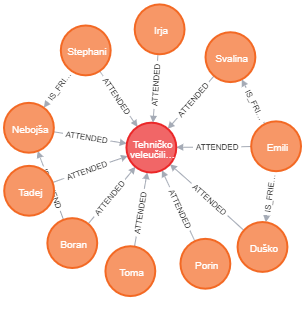
\includegraphics[scale=0.7]{slike/same_college.png}
		\caption{Studenti \emph{TVZ}-a}
		\label{fig:common_friends}
	\end{figure}
	
	Ovo su neke od metoda koje se mogu koristiti za preporuke u društvenim mrežama te su poslužile kao inspiracija za upite kojima aplikacija predlaže korisnicima njihove potencijalne prijatelje. \\
	Dio projekta bio je osmisliti upite koji će predlagati prijatelje na temelju znanja i obrazovanja te za osobne preporuke.
	
	\subsection{Poslovne preporuke}
	Želja je omogućiti korisniku brzo i efikasno umrežavanje sa ljudima istih ili sličnih vještina. \\
	Izglednije je da će korisnik dodati osobu sličnih vještina zbog mogućnosti suradnje. Ovo podosta zvuči kao klasifikacijska preporuka, no je li moguće dodatno personalizirati preporuke na temelju postojećih informacija? \\
	Očito je korisniku važno upoznati ljude sa srodnih fakulteta. To će biti prvi filter preporuka.\\
	Upit je prezentiran u koracima. \\
	U idućem upitu primjetite nizove znakova nakon dolara. To su vrijednosti koje korisnik predaje prilikom slanja upita. Ako je aplikaciju uključila osoba sa identifikacijskim brojem $14$ tada će se idući upit izvršiti s tim identifikacijskim brojem.
	
	\begin{samepage}
		\begin{minted}[tabsize=1,breaklines]{java}
			MATCH (p:Person {id:$id})-[:ATTENDED]->(:College)-[:SAME_AREA]-
			(:College)<-[:ATTENDED]-(recommendation:Person)
			WHERE p.id <> recommendation.id AND NOT((p)-[:IS_FRIEND]-(recommendation))
			
		\end{minted}
	\end{samepage}
	Idući dio ovisi o korisniku. Ljudi različitog godišta imaju različite poslovne interese. \\
	Mlađi ljudi će zbog srama, neiskustva i sličnog teže pristupiti  iskusnijoj osobi. Izglednije je da će mlađa osoba htjeti dodati svoje vršnjake koji imaju slična iskustva. \\
	S druge strane iskusnija osoba mari manje za to i više ju zanimaju vještine korisnika. Na primjer poslodavcu može biti zanimljivo zaposliti studenta kao ulaganje u budućnost, ali može mu od interesa biti i zapošljavanje iskusnih ljudi iz njegovog područja. \\
	Dakle idući filter za mlade ljude bit će razlika u godinama, što je manja izglednije je da će joj se ta osoba preporučiti dok će za starije ljude filter biti presjek istih vještina koje osoba ima. \\
	Sada kada su preporuke dodatno sužene, ako je to potrebno, opet po godištu dodajemo nove filtere. \\
	U ovom slučaju ćemo zamijeniti uloge. Mlađi ljudi će sada u svojem popisu preporuka imati ljude sličnog godišta pa će se te preporuke filtrirati po presjeku vještina zato što je izglednije da će mladi ljudi htjeti dodati osobu zainteresiranu za njihovo područje. \\
	Starijim korisnicima filter će djelovati suprotno od filtera za mlađe korisnike. Preporuke će poredati po razlici u godinama kako bi im predstavili najiskusnije ljude iz njihovog područja. \\
	Slijedi nastavak na prethodni komad koda sastavljen od navedena dva filtera za starije korisnike:
	\begin{samepage}
		\begin{minted}[tabsize=1,breaklines]{java}
			WITH p, recommendation, size([x IN p.skills WHERE x IN recommendation.skills]) AS common_skills 
			ORDER BY common_skills DESC LIMIT $first_limit
			RETURN recommendation, abs(p.date_of_birth.year - recommendation.date_of_birth.year) AS birth_delta 
			ORDER BY birth_delta DESC LIMIT $limit;
			
		\end{minted}
	\end{samepage}
	\newpage
    \begin{samepage}
    Rezultat sljedećeg upita za korisnicu Lori Vulin vidljiv je na grafičkom sučelju:
    
    \begin{figure}[h!]
        \centering
        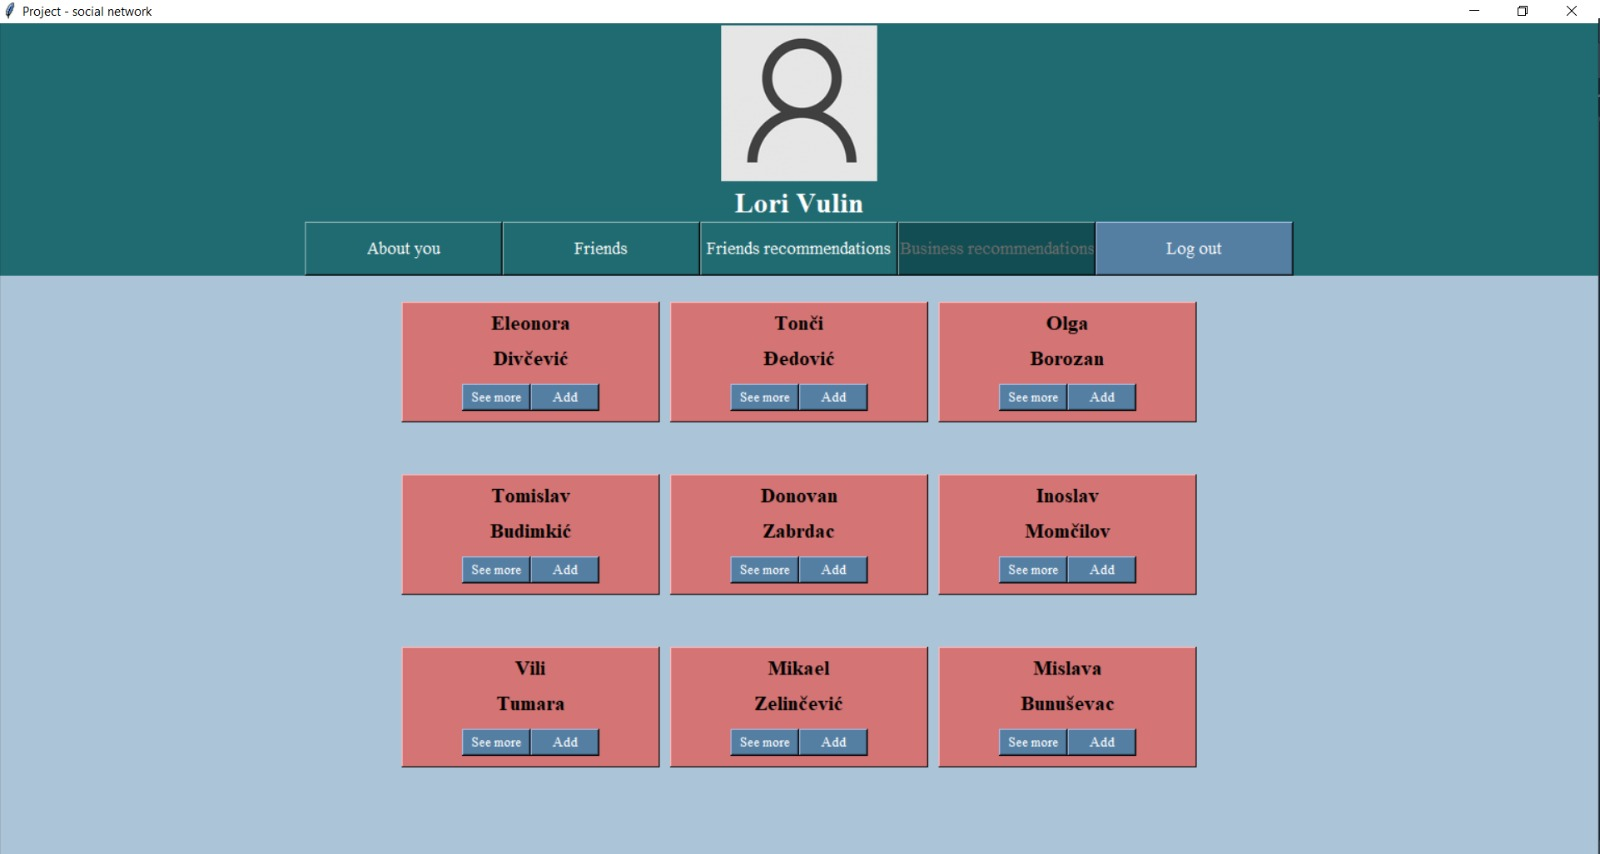
\includegraphics[scale=0.4]{slike/business.jpg}
        \caption{Poslovne preporuke}
        \label{fig:business_rec}
    \end{figure}
    
    \subsection{Osobne preporuke}
    Slično kao poslovne preporuke osobne preporuke se odvijaju u nekoliko koraka. \\
    Prvi korak je odabir osoba sa najviše zajedničkih prijatelja kako bi postojala veća vjerojatnost poznanstva.
    \begin{samepage}
    \begin{minted}[tabsize=1,breaklines]{java}
    MATCH (p:Person {id:$id})-[:IS_FRIEND]-(:Person)-[:IS_FRIEND]-(recommendation:Person)
    WHERE p.id <> recommendation.id AND NOT((p)-[:IS_FRIEND]-(recommendation))
    WITH p, recommendation, count(recommendation) AS common_friends
    ORDER BY common_friends DESC LIMIT $first_limit
    
    \end{minted}
    \end{samepage}
    
    \end{samepage}
	Ovoga puta je drugi korak za sve isti. Ljudi se češće druže sa ljudima svojeg godišta pa idući filter odabire najbliže ljude po godištu:
	\begin{samepage}
		\begin{minted}[tabsize=1,breaklines]{java}
			WITH p, recommendation, abs(recommendation.date_of_birth.year - p.date_of_birth.year) AS birth_delta 
			ORDER BY birth_delta LIMIT $second_limit
			
		\end{minted}
	\end{samepage}
	
	Finalno potrebno je provjeriti kombatibilnost korisnika. Sada je osim presjeka vještina u obzir uzet i presjek hobija. \\
	Očito može biti važno da ljudi imaju iste vještine s obzirom da iz toga često proizlaze poznanstva, ali istom logikom važan je i presjek hobija. \\
	Ako se dvoje ljudi bavi istom aktivnosti u slobodno vrijeme izgledno je da bi se mogli slagati ili se već poznaju. \\
	Ovime se finalizira upit koji za osobne preporuke ljudima:
	\begin{samepage}
		\begin{minted}[tabsize=1,breaklines]{java}
			RETURN recommendation, size([skill IN p.skills WHERE skill IN recommendation.skills]) + size([hobby IN p.hobbies WHERE hobby IN recommendation.hobbies]) AS common 
			ORDER BY common DESC LIMIT $limit;
			
		\end{minted}
	\end{samepage}
	\newpage
	\begin{samepage}
		Rezultate upita moguće je vidjeti na grafičkom sučelju:
		\begin{figure}[h]
			\centering
			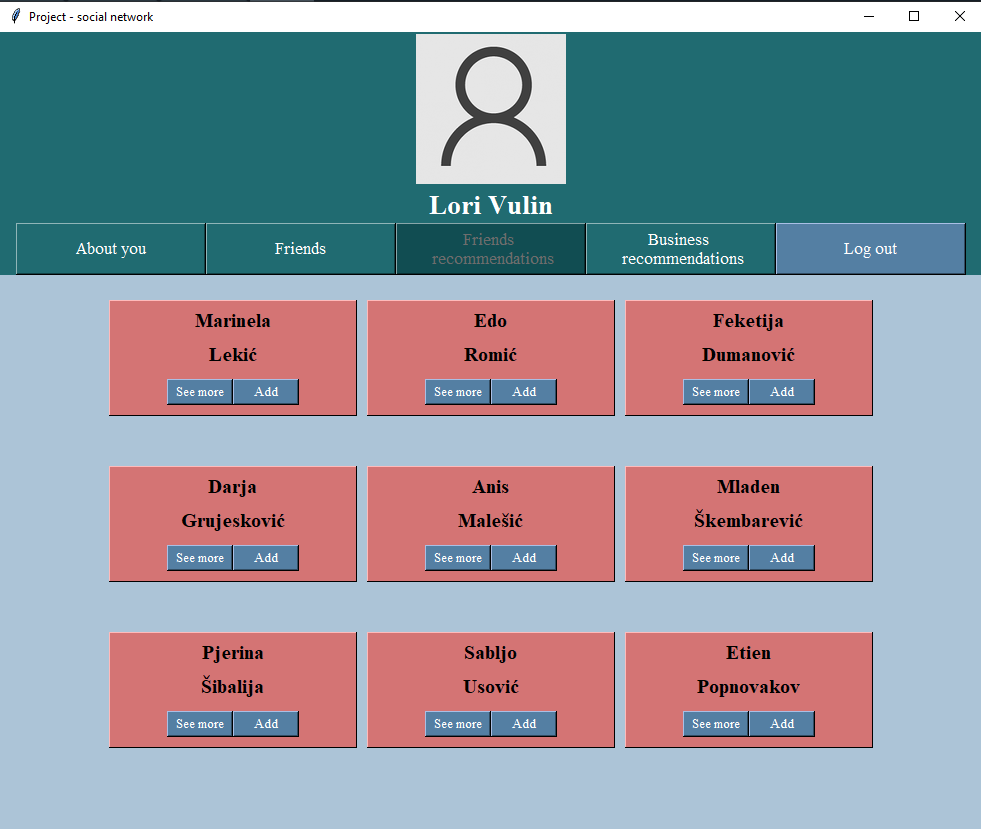
\includegraphics[scale=0.4]{slike/personal.jpg}
			\caption{Osobne preporuke}
			\label{fig:personal_rec}
		\end{figure}
	\end{samepage}
	
	\subsection{Brzina izvršavanja upita}
	Zanimljiva stvar koja je uočena prilikom stvaranja aplikacije je neovisnost trajanja upita o veličini baze. Odabrani su najsloženiji upiti, što su upravo upiti za preporučavanje prijatelja te se \emph{Pythonovom} bibliotekom \emph{time} mjerilo vrijeme izvršavanja svakog upita. \\
	Napravljeno je po deset baza za svaku od veličina iz skupa $\{50, 100, 150, \dots, 1000\}$ gdje elementi skupa predstavljaju broj osoba koji se nalaze u bazi podataka. Za svaku od tih baza upit je poslan za tri nasumično odabrana korisnika te su dobijeni sljedeći rezultati.\\
	
	\begin{figure}[h]
		\centering
		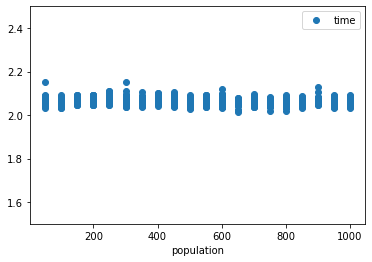
\includegraphics[scale=0.5]{slike/personal_graph.png}
		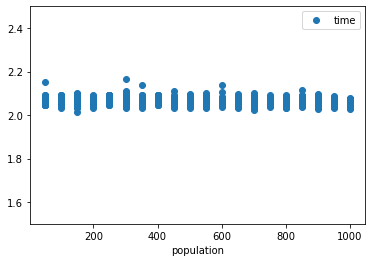
\includegraphics[scale=0.5]{slike/business_graph.png}
		\caption{Brzina upita}
		\label{fig:query_speed}
	\end{figure}
	
	
	Iznenađujuće, vrijeme izvršavanja upita ostaje konstantno te traje nešto više od dvije sekunde. \\
	Iako na prvu ruku rezultat izgleda neočekivano razlog u tome nalazimo na naviku korištenja relacijskih baza podataka. Tamo bi bilo potrebno raditi Kartezijev produkt tablica što bi dovelo do značajno sporijeg vremena izvršavanja. Dobro je napomenuti da bi i taj upit bio značajno kompliciraniji i manje čitak. \\
	Međutim ovdje ne dolazi do Kartezijevog produkta već se pretraživanje odvija grafovskim algoritmima što daje veliko ubrzanje.
	
	
	\newpage
	\section{Korištenje aplikacije}
	Nakon opisanih tehnologija, strukture podatka i upita koje koristimo, u ovome ćemo Vas odjeljku provesti kroz korištenje same aplikacije. 
	
	\subsection{Početni zaslon, zaslon za ulogiravanje i registriranje}
	Pokretanjem aplikacije pokreće se prozor koji nudi mogućnost odabira \emph{ulogiravanja} ili \emph{registriranja}. Klikom na gumb \emph{Register} iscrtava se novi prozor koji predstavlja formu u koju korisnik unosi svoje podatke potrebne za registraciju. 
	
	Sve dijelove forme obavezno je popuniti pri registraciji. Dijelovi forme koje korisnik mora (korektno) popuniti su:
	\begin{itemize}
		\item ime i prezime: vrijednosti koje korisnik unosi moraju biti sastavljene samo od slova, ako je korisnik već u bazi dobit će prikladnu poruku
		\item spol: bira se klikom na dvije ponuđene vrijednosti
		\item datum rođenja: pronalazi se korištenjem kalendara, moguće je kretati se po mjesecima ili godini te odabrati određeni dan, nisu prikazani datumi koji nisu dozvoljeni u bazi
		\item fakultet: bira se jedan među ponuđenima
		\item godina upisa: unos godine koje je korisnik krenuo na fakultet, mora biti veća od godine rođenja uvećane za 18
		\item godina završetka: unos godine koje je korisnik završio fakultet ili u slučaju da još studira koje ga godine planira završiti, razlika godina upisa i završetka mora biti između 5 i 10 godina da bi unos bio korektan
		\item ocjena: unos prosjeka ocjena na fakultetu, mora biti decimalni broj koji je veći ili jednak 2.00 i manji ili jednak 5.00.
	\end{itemize}
	
	Klikom na gumb provjeravaju se dotad unešene vrijednosti i u slučaju greške u skočnom prozoru piše opis greške pri unosu. 
	
	Ukoliko su sve vrijednosti ispravno unesene, pojavljuje se lista s vještinama koje su predodređene za fakultet koji je korisnik izabrao (Slika ~\ref{fig:forma}). Klikom miša na vještinu ona postane označena i moguće je na taj način označiti proizvoljan broj vještina koje će se pridodati korisniku pri registraciji u bazu. Kada je završio s odabirom klikne na gumb i ponovi postupak na listi svih hobija koji se nalaze u bazi. 
	
	Korisnik mora izabrati barem jedan hobi i bar jednu vještinu, u suprotnom iskoči prozorčić s porukom. 
	
	Klikom na gumb, uz pretpostavku da je sve korektno upisano, pojavljuje se poruka da je registracija uspijela. Korisnik je sada registriran i upisan u bazu. Kako bi koristio aplikaciju mora zatvoriti prozore \emph{Register} i skočni prozor te se \emph{ulogirati}.
	
	Za ulogiravanje je potrebno kliknuti gumb \emph{Log in} i u formu upisati ime i prezime. Ako podaci nisu ispravno zadani ili se korisnik ne nalazi u bazi dobije se prikladna poruka. (Slika~\ref{fig:login}) Korektnim unosom ulazimo u glavni dio aplikacije. 
	
	\begin{figure}
		\begin{center}
			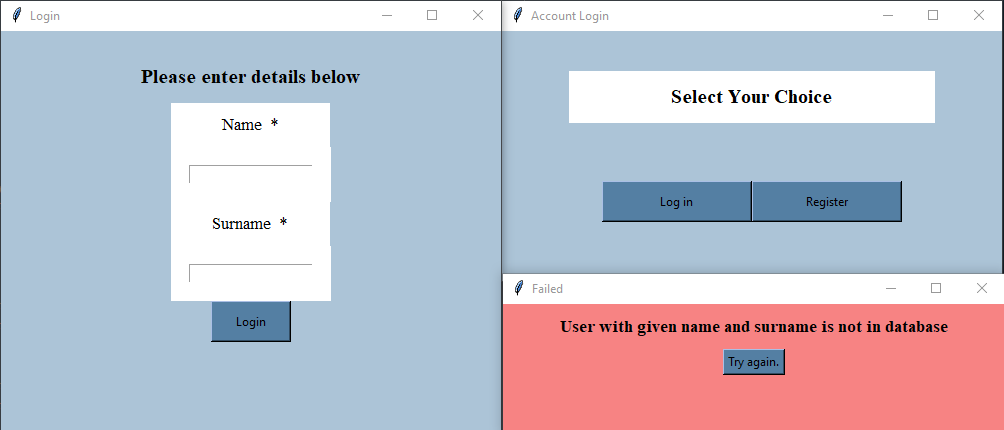
\includegraphics[scale=0.5]{slike/login.png}
			\caption{Login, početni prozor i skočni prozor s greškom}
			\label{fig:login} 
		\end{center}
	\end{figure}
	
	\subsection{Stranica s informacijama}
	
	Ulaskom u aplikaciju otvara se stranica o ulogiranom korisniku, izgledom kao na slici~\ref{fig:info}. Ona se sastoji od nekoliko dijelova, gornji dio (\emph{header}) sastoji se od ikone, imena i prezimena korisnika te izbornika. Izbornik je uređen kao lista gumbova, stoga klikom na njih se otvara nova kartica u ovisnosti o tome koju karticu želimo vidjeti. Kako se trenutno nalazimo na kartici \emph{About you}, gumb koji inače omogućuje odlazak na ovu stranicu je trenutno onemogućen. 
	
	Ispod izbornika ispisane su informacije o korisniku. Kako ne bi sve bilo monotono, dodan je pravokutnik \emph{Gender} obojan u boju (plavu ili crvenu) u ovisnosti o vrijednosti koju ispisuje. 
	
	\begin{figure}
		\begin{center}
			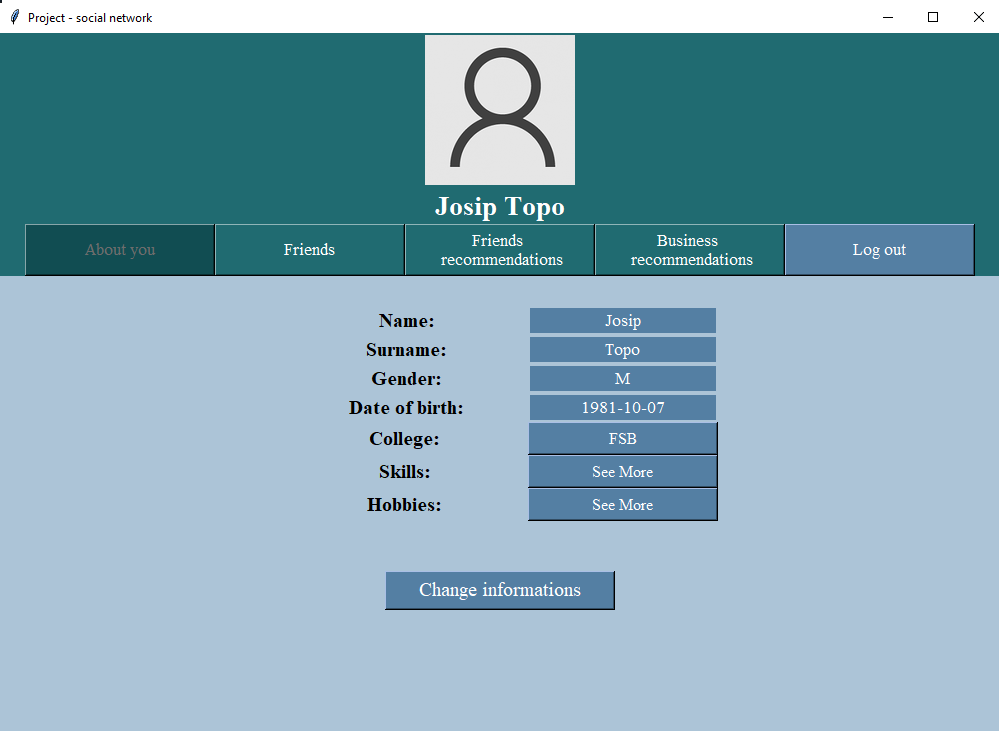
\includegraphics[scale=0.45]{slike/info.png}
			\caption{Kartica s informacijama o korisniku}
			\label{fig:info} 
		\end{center}
	\end{figure}
	Prikaze detalja o fakultetu, vještinama i hobijima realizirali smo tako što se pritiskom na gumb iscrtava prozor koji sadrži željene informacije. Svaki od njih sadrži i gumb za gašenje prozorčića. Sve opisano možete proučiti na slici~\ref{fig:coll_info}.
	
	\begin{figure}
		\begin{center}
			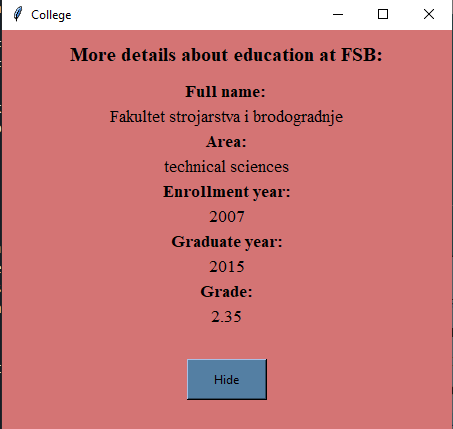
\includegraphics[scale=0.9]{slike/coll_info.png}
			\caption{Informacije o fakultetu i studiranju korisnika}
			\label{fig:coll_info} 
		\end{center}
	\end{figure}
	
	\subsubsection{Mjenjanje podatka}
	
	Na dnu stranice s informacijama postoji mogućnost promjene nekih podataka. To je dodatna funkcionalnost koju smo odlučili implementirati kako bi poboljšali korisnikovo iskustvo korištenja aplikacije. Međutim, nismo smijeli dopustiti promjenu nekih podatka ili unos pogrešnih informacija.  
	
	Kako bi se podaci promjenili potrebno je upisati koju informaciju mijenjamo i novu vrijednost kojom je mjenjamo.(Slika~\ref{fig:change} Moguće je promjeniti ove informacije(potrebno je unijeti ključnu riječ točno kao što je navedeno):
	\begin{samepage}
		
		
		\begin{itemize}
			\item \textbf{name} - mjenja ime, provjera se je li sastavljeno samo od slova i je li već postoji netko u bazi s kombinacijom novog imena i starog prezimena, ako da nije moguće izvršiti promjenu
			\item \textbf{prezime} - mjenja prezime, analogno kao i za ime ostalo
			\item \textbf{graduate year} - mjenja godinu završetka fakulteta, korisno ukoliko je osoba u međuvremenu položila fakultet, vrši s provjera je li korektno u odnosu na godinu početka studija
			\item \textbf{grade} - mjenjanje ocjene, korisnik mora paziti na ocjena bude napisana u obliku x.yy, gdje je ocjena veća ili jednaka 2.0 i manja ili jednaka 5.0 
		\end{itemize}
	\end{samepage}
	
	\begin{figure}
		\begin{center}
			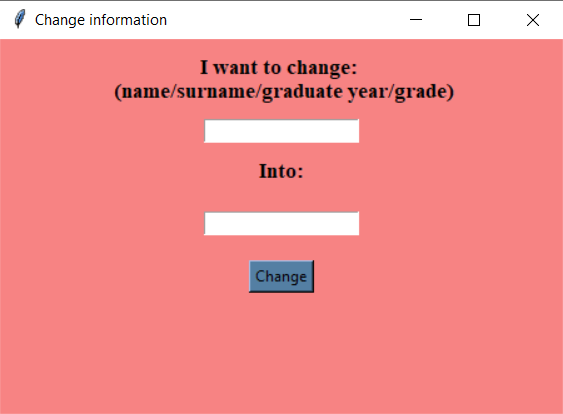
\includegraphics[scale=0.9]{slike/change.png}
			\caption{Prozor za promjenu podataka}
			\label{fig:change} 
		\end{center}
	\end{figure}
	
	Ukoliko je neki od podataka kriv ispisat će se odgovarajuća poruka, a u suprotnom na kartici informacije promjenit će se podaci. 
	
	\subsection{Kartica prijatelji}
	
	Kartica prijatelji nudi mogućnost uvida korisnikovih prijatelja i pretraživanja liste prijatelja po nekim svojstvima.
	Osim elemenata \emph{headera} imamo i poseban dio gdje korisnik treba odabrati jednu od ponuđenih opcija. Opcije koje su ponuđene predstavljaju način na koji će se tražiti ljudi iz baze s kojima je korisnik prijatelj. Odnosno, prijatelje možemo tražiti po imenu, prezimenu, godini rođenja, fakultetu, godinu upisa ili završetka. Nakon što smo odabrali opciju po kojoj tražimo prikazat će nam se forma za unos teksta u koji ćemo onda upisati ključnu riječ po kojoj pretražujemo. Taj se dio neće ispisati ukoliko smo odabrali \emph{All} opciju. Mala napomena je da je kod pretraživanja po fakultetu u formu potrebno upisati kratko ime fakulteta.
	
	
	\begin{figure}
		\begin{center}
			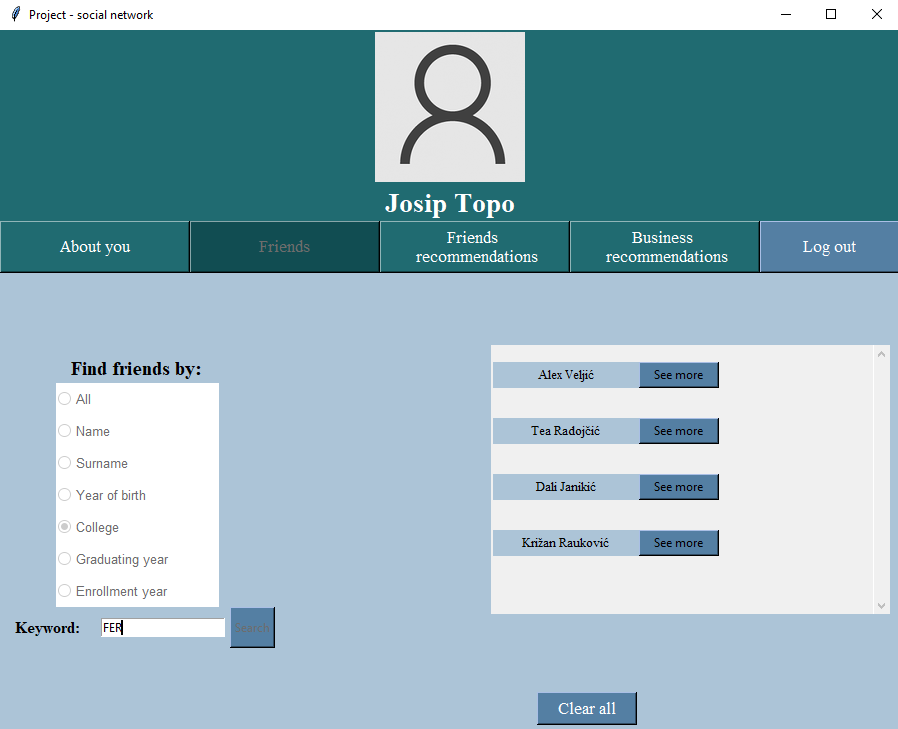
\includegraphics[scale=0.5]{slike/search.png}
			\caption{Kartica prijatelji}
			\label{fig:search} 
		\end{center}
	\end{figure}
	
	Nakon što pokrenemo traženje imamo dva scenarija. Prvi je da se ne pronalazi prijatelj u bazi pa se ispisuje prikladna pogreška, dok je drugi da se ispise element koji je \emph{skrolabilan} i u kojem su ispisana imena i prezimena osoba zajedno s gumbićem. (vidi sliku~\ref{fig:search}) Operacija koja se poziva klikom na gumb je pozivanje prozora u kojem se na jednom mjestu ispisuje sve bitno o odabranoj osobi.
	
	U svakom je trenutku omogućen gumb \emph{Clear all}. Kliknemo li na njega izbrisat će nam se sve što smo imali na ekranu i vraćamo se na početni izgled ekrana s ponuđenim opcijama po kojima tražimo prijatelje.
	
	%razmisljala sma mozda dodat ili ako budu pitali reci recenicu da se analogno moglo dodat za sve osobe i omogucit dodavanje prijatelja, ali kako je ovo opcionalni dio aplikacije odlucili smo se demonstrirati ga na ovome mjestu, no svakako se kasnije moze dodat jos jedna kartica s tom mogućnosti
	
	\subsection{Kartice preporuka}
	
	Ostale su nam još dvije stranice koje nismo opisali, a veoma su sličnih funkcionalnosti, kao i izgleda, pa ih zato opisujemo skupa. Svaka od njih sadrži izbornik i u središnjem dijelu prikaz osoba koje je korisnik dobio kao preporučene. One su dobivene pozivom upita o preporukama koje su opisane u prethodnom poglavlju. Za svaku osobu osim imena i prezimena imamo dva gumba, jedan nas vodi na prozor u kojem su ispisane sve informacije o osobi, dok se klikom na drugi gumb dodaje prijateljstvo između korisnika i osobe čiji je gumb korisnik stisnuo.
	
	Nakon što se klikne gumb i doda prijateljstvo u bazu, gumb \emph{Add} postaje onemogućen. Odlaskom s kartice i kasnije ponovim ulaskom na nju, osobe koju smo prethodno dodali nema na prikazu, već se predlažu nove osobe koje nam još nisu prijatelji. Primjer kartice smo prikazali na slici~\ref{fig:business_rec}.
	
	Za kraj spomenimo da se korisnik može u svakom trenutku \emph{izlogirati} iz aplikacije i ponovo se vratiti na početni prozor. Također, nismo htjeli dodatno komplicirati bazu, no nije teško dodati dio autentifikacije korisnika pri ulasku u aplikaciju. Tada bi umjesto imena i prezimena korisnik ulazio u aplikaciju upisujući korisničko ime i pripadnu lozinku. 
	
	\section{Zaključak}
	U ovome smo projektome zadatku uz korištenje \emph{Neo4j-a} i istoimenog modula u \emph{Pythonu} izgradili aplikaciju za interakciju sa bazom podataka \emph{Neo4j}. Baza pohranjuje podatke kakve bi mogli pronaći u društvenoj mreži. Realizirali smo upite pomoću kojih osobama dajemo preporuke  prijatelja na temelju poslovnih i osobnih karakteristika. Za potrebe aplikacije i zadatka izgenerirali smo podatke i njima napunili bazu. Omogućili smo dodavanje novih korisnika te osigurali konzistentnost podataka koje korisnik unosi. Programski kod koji smo pisali može se pronaći na \href{https://github.com/basioli-k/social_network}{\emph{repozitoriju}}. Također, spomenuli bi kako je moguće prirodno obogatiti bazu raznim vrhovima i bridovima. Smisleno bi bilo dodati firmu u kojoj korisnici se korisnici mogu zaposliti. To ovdje nije napravljeno jer smo smatrali da na ovaj način možemo prikazati dovoljno zanimljivih aspekata korištenih tehnologija. \\
	Svoje znanje \emph{Pythona} smo uvelike nadogradili i vidjeli koliko truda je potrebno za izradu čak i jednostavnog modela društvene mreže. \emph{Neo4j} pokazao se kao učinkovit i intuitivan izbor baze podataka za ovakav problem u odnosu na druge baze podataka zbog načina na koji tretira veze između korisnika. 
	
	
	\newpage
	\nocite{*}
    \printbibliography
\end{document}
